\documentclass[times,specification,annotation]{itmo-student-thesis}

%% Опции пакета:
%% - specification - если есть, генерируется задание, иначе не генерируется
%% - annotation - если есть, генерируется аннотация, иначе не генерируется
%% - times - делает все шрифтом Times New Roman, собирается с помощью xelatex
%% - pscyr - делает все шрифтом Times New Roman, требует пакета pscyr.

%% Делает запятую в формулах более интеллектуальной, например:
%% $1,5x$ будет читаться как полтора икса, а не один запятая пять иксов.
%% Однако если написать $1, 5x$, то все будет как прежде.
\usepackage{icomma}

%% Один из пакетов, позволяющий делать таблицы на всю ширину текста.
\usepackage{tabularx}

\usepackage{tikz}

\usetikzlibrary{arrows.meta, fit, automata, positioning}

\usepackage{mathtools}

\usepackage{makecell}

\graphicspath{ {./images/} }

%% Указываем файл с библиографией.
\addbibresource{bachelor-thesis.bib}

\begin{document}

\studygroup{M3439}
\title{Обучение метрики похожести сообществ с помощью выделения
векторного представления}
\author{Зернов Глеб Сергеевич}{Зернов Г.С.}
\supervisor{Сметанников Иван Борисович}{Сметанников И.Б.}{к.техн.н.}{ассистент, факультет информационных технологий и программирования, Университет ИТМО}
\publishyear{2019}
%% Дата выдачи задания. Можно не указывать, тогда надо будет заполнить от руки.
\startdate{18}{декабря}{2018}
%% Срок сдачи студентом работы. Можно не указывать, тогда надо будет заполнить от руки.
\finishdate{6}{мая}{2019}
%% Дата защиты. Можно не указывать, тогда надо будет заполнить от руки.
\defencedate{}{}{2019}

\addconsultant{Попов А.Л.}{магистр}

\secretary{Павлова О.Н.}

%% Задание
%%% Техническое задание и исходные данные к работе
\technicalspec{Разработать модель, которая позволит представить сообщества социальной сети в
виде векторов. Модель необходимо обучить и протестировать на анонимных неразмеченных
сессионных данных из социальной сети «Вконтакте». Необходимо проанализировать
результаты и сравнить предлагаемое решение с альтернативными методами.}

%%% Содержание выпускной квалификационной работы (перечень подлежащих разработке вопросов)
\plannedcontents{
\begin{enumerate}
\item[1.] Описание предметной области. Обзор существующих алгоритмов.
\item[2.]  Описание алгоритма векторного представления сообществ
\item[3.]  Анализ результатов, сравнение с существующими решениями.
\end{enumerate}}

%%% Исходные материалы и пособия 
\plannedsources{}

%%% Цель исследования
\researchaim{Реализация алгоритма представления сообществ социальной сети в виде векторов.}

%%% Задачи, решаемые в ВКР
\researchtargets{\begin{enumerate}
    \item Обзор существующих подходов.
    \item Разработка алгоритма
выделения векторного представления сообществ по сессионным анонимным неразмеченным
данным. 
    \item Анализ полученных результатов.
\end{enumerate}}

%%% Использование современных пакетов компьютерных программ и технологий
\addadvancedsoftware{Язык программирования \texttt{Python}}{
    \ref{sec:algo-subs} - \ref{sec:visual}
}
\addadvancedsoftware{Программное средство \texttt{Jupyter Notebook}}{\ref{sec:algo-subs} - \ref{sec:visual}}
\addadvancedsoftware{Библиотека \texttt{Pytorch}}{\ref{sec:algo-subs} - \ref{sec:algo-combined}}
\addadvancedsoftware{Библиотека \texttt{Sklearn}}{\ref{sec:class}, \ref{sec:visual}}
\addadvancedsoftware{Библиотека \texttt{Matplotlib}}{\ref{sec:visual}}
\addadvancedsoftware{Библиотека \texttt{Spark} и язык программирования \texttt{Skala}}{\ref{sec:class}}

%%% Краткая характеристика полученных результатов 
\researchsummary{Исследованы существующие решения данной задачи. Реализован алгоритм, позволяющий
решить поставленную задачу. Проведено сравнение предложенного решения с существующими
путем решения дополнительных задач классификации с использованием результатов работы
моделей в качестве входных данных.}

%%% Гранты, полученные при выполнении работы 
\researchfunding{При выполнении работы грантов получено не было.}

%%% Наличие публикаций и выступлений на конференциях по теме выпускной работы
\researchpublications{Нет}

%% Эта команда генерирует титульный лист и аннотацию.
\maketitle{Бакалавр}

%% Оглавление
\tableofcontents

%% Макрос для введения. Совместим со старым стилевиком.
\startprefacepage

\startrelatedwork

Обычно объекты из реального мира представимы в виде набора некоторого
количества признаков, численные значения которых, в свою очередь, можно
представить в виде вектора. Таким образом, мы можем получить представление о
положении объектов относительно друг друга в полученном пространстве,
сохраняя при этом знания о конкретных признаках каждого объекта. Такие
векторы можно использовать в ряде алгоритмов машинного обучения, исходя из
простого правила: чем ближе два вектора друг к другу, тем более похожи между
собой два объекта семантически.

Однако, существует возможность столкнуться с рядом проблем при попытке
представить объекты в виде векторов. К примеру, полученные векторы могут не
коррелировать с положением дел в реальном мире. В таком случае, выбранные
нами векторы не подходят для алгоритмов машинного обучения, поскольку
алгоритм не будет способен сопоставить положение векторов в пространстве с картиной
реального мира. Кроме того, какие-то сущности имеют либо слишком большое
число признаков, и понять, какие признаки стоит добавить в конечный вектор, а
какие отбросить, бывает крайне трудной задачей.

Решением этих проблем выступают модели представления объектов в виде векторов, позволяющие описывать объект и его свойства.

Полученные векторы имеют практическую ценность. Например, они могут быть использованы в
качестве входных данных другой модели и проанализированы с целью
получить представление о сходстве пар объектов между собой. Такие векторы содержат большое количество информации в сжатом виде, в отличие, от, например, классического one-hot векторного представления объектов.

Алгоритмы векторного представления объектов получили широкое распространение и используются в различных областях. Например, социальная сеть Pinterest\footnote{https://www.pinterest.com} \cite{Liu2017} использует модель векторизации объектов социальной сети (Pin'ов), сервис YouTube\footnote{https://youtube.com} использует алгоритмы векторного представления для рекомендации видео\cite{Covington2016} 

В данной работе рассматриваются алгоритмы построения такого представления для сообществ социальной сети. Во второй главе описывается модель, позволяющая строить векторные представления сообществ по сессионным данным пользовательской активности. Рассматриваются три вариации алгоритма: базовая, позволяющая работать с позитивными и негативными редкими откликами пользователя, альтернативная, работающая со слабыми и частыми сигналами и комбинированная, учитывающая оба типа пользовательской активности. В заключительной главе проводятся эксперименты по сравнению предложенных алгоритмов с альтернативными вариантами, а также сравниваются варианты конечной модели между собой. 

%% Начало содержательной части.
\chapter{Описание предметной области}

«Вконтакте»\footnote{https://vk.com} --- одна из крупнейших социальных сетей СНГ и самая
популярная соц. сеть в России. «Вконтакте» на ряду с многими другими
социальными сетями имеет внутри себя объединения пользователей по интересам,
называемое сообществами. Пользователи имеют возможность подписаться на
интересуемое их сообщество для более удобного взаимодействия с информацией
сообщества, а также отписаться от него. Сообщества могут добавлять на свою
страницу записи (текст, картинки, видео и т. д.), которые пользователи могут
помечать как понравившиеся («лайки»), комментировать и прочее.

Существенной сложностью работы с сообществами является число сообществ (миллионы), каждое из которых может состоять из миллионов пользователей, и содержать миллионы записей.  

Таким образом, полная информация о сообществе --- это огромный массив
данных, предоставляя который полностью некоторой модели машинного обучения,
мы не только существенно увеличиваем размер необходимого объёма памяти для хранения этой информации, но и замедляем работу самого алгоритма, что делает алгоритм бесполезным для применения на практике.

Выходом из этой ситуации является некоторое более ёмкое представление сообщества без потери интересующей нас информации.

Главная задача, решаемая в моей работе, --- разработать алгоритм выделения универсального векторного представление сообществ небольшой размерности. 

\section{Основные определения}

%TODO: больше определений и вводных понятий

%Векторное представление или эмбеддинг (англ. Embedding) --- отображение
%множества объектов на пространство векторов с сохранением некоторой
%структуры за объектами.

\section{Постановка задачи}\label{sec:intro}

Формализуем поставленную задачу: для заданного множества $C$ сообществ, пользователей $N$ и сессий пользовательской активности $A_n$, $n \in N$ найти представление $v_{c} \in \mathbb{R}^d$ размерности $d$ для каждого сообщества $c \in C$ так, что семантически похожие сообщества находятся близко друг к другу в конечном векторном пространстве. 

Данная задача решается для 3 случаев представления сессий $A_n$
 
В первом случае сессия состоит из множества событий двух типов:
 \begin{align}
A_n = (S_n, U_n) 
\label{eq-subs}
\end{align}
Где события $S_n$ --- список последовательных $K$ уникальных подписок на сообщества пользователя $n$ за некоторый промежуток времени: $S_n = (c_{1}, c_{2}, \dots, c_{K}), \forall i \ne j : c_i \ne c_j$, а $U_n$ --- список последовательных $M$ уникальных отписок от сообществ пользователя $n$: $U_n = (c_{1},  c_{2}, \dots, c_{M}), \forall i \ne j : c_i \ne c_j$, $S_n \cap U_n = \varnothing$.

Во втором случае сессия задаётся как множество $K$ (не обязательно уникальных) действий (<<лайков>>) пользователя $n$ записей сообществ:
 \begin{align}
A_n = (c_{1}, c_{2}, \dots, c_{K}) 
\label{eq-likes}
\end{align}
 
В третьем случае каждой сессии задаётся тип $T_n$ пользовательских событий, представленных в ней $T_n = \{subs, likes\}$ --- подписки/отписки, либо лайки. В таком случае сессия задается в зависимости от типа:
\begin{equation}
    A_n =
    \begin{cases}
      (S_n, U_n), & \text{if}\ T_n=subs \\
      (c_{1}, c_{2}, \dots, c_{K}), & \text{if}\ T_n=likes
    \end{cases}  
    \label{eq-combined}
  \end{equation}
 И определяется формулой (\ref{eq-subs}) для первого типа, формулой (\ref{eq-likes}) для второго.

\subsection{Формат входных данных}

Компанией были предоставлены анонимные сессионные действия пользователей за небольшой промежуток времени. Всего было предоставлено 3 набора данных.

Первый набор данных состоит из списка сессий, каждая сессия --- это список действий некоторого пользователя, элементами списка является идентификатор сообщества (id) и маркер действия (подписка/отписка). Данные были собраны по действиям пользователей за 2-3 месяца.

Также были предоставлены сессионные данные по <<лайкам>> пользователя в аналогичном формате: список сессий, каждая сессия является списком id сообществ, запись которого понравились пользователю. Как было отмечено ранее, в отличие от данных по подпискам, в сессии по лайкам сообщество может встречаться несколько раз. Данные были собраны по действиям пользователей за 2-3 дня. Таким образом, средняя длина сессий второго набора данных примерно равна средней длины сессий из первого набора данных. 

Третий набор данных является комбинацией из первых двух, каждая сессия имеет тип того, какая информация в ней содержится: действия пользователя по подпискам или лайкам. 

После фильтрации данных общее число сессий было сокращено до 500 000 (450 000 сессий в первом наборе данных), число уникальных групп до 11 200 для каждого набора данных. Средняя длина сессий всех наборов данных примерно равна 4.5

\section{Обзор существующих решений}

\subsection{Алгоритм факторизации матриц в рекомендательных системах.}\label{sec:als}

Персонализация пользовательского контента является одной из основополагающих частей систем, предоставляющих такой контент конечным пользователям. Лидеры интернет-торговли или интернет-услуг особенно заинтересованы в таких алгоритмах, поскольку позволяет увеличить пользовательский отклик.
В общем случае, рекомендательные системы берут за основу две стратегии: фильтрация контента (content filtering) \cite{Lops2011,} и коллаборативная фильтрация (collaborative filtering)
  
Главная идея за фильтрацией контента состоит в том, чтобы создать профиль для каждого пользователя или продукта с целью охарактеризовать сущность. Например, в качестве профиля фильма могут выступать жанр, актёры, кассовые сборы и т.д.

Альтернативный вариант, коллаборативная фильтрация, опирается на действия пользователей, сделанных в прошлом. Такие алгоритмы анализируют статистические связи между пользователями, продуктами, их взаимодействиями и дают рекомендации, основываясь на исторических данных.  Большим плюсом таких систем является независимость от домена, в котором они применяются.

Одним из самых распространённых на данный момент времени алгоритмов в сфере рекомендательных систем является алгоритм факторизации матриц \cite{koren2009}, относящийся к группе алгоритмов коллаборативной фильтрации.

Модель матричной факторизации переносит пользователей и продукты в пространство признаков размерности $n$. Таким образом, продукт $p$ представим в виде вектора $a_{p} \in \mathbb{R}^n$ , а пользователь $u$ в виде вектора $b_{u} \in \mathbb{R}^n$. Для продукта каждый из элементов вектора отвечает за то, насколько каждый признак характерен для  этого продукта. В то время для пользователя элементы вектора показывают, насколько пользователю интерес признак.

Это позволяет задать оценку пользователя $u$ продукта $p$ в виде формулы
 \begin{align*}
r_{ui} = a_{i}^{T}b_{u}
\end{align*}
Таким образом, зная матрицу пользовательских оценок $R$ можно разложить ее на произведение матриц $A$ и $B$, отвечающих за векторное произведение продуктов и пользователей соответственно.
 \begin{align*}
R = A^TB
\end{align*}

В рамках задачи, поставленной формулой(\ref{eq-subs}), составим матрицу оценок следующим образом: для подписки пользователя $i$ на сообщество $j$ поставим единицу на эту позицию $R_{ij} = 1$, аналогично для отписки $R_{ij} = - 1$. В случае отсутствия действий пользователя для сообщества оценка будет равна нулю.

Адаптируя алгоритм ALS для представления сессий формулы (\ref{eq-likes}), мы можем представить оценку пользователя сообществу, как число <<лайков>>, которые он поставил этому сообществу за сессию.

Для работы с комбинированными данными (формула \ref{eq-сombined}), соединим эти два подхода. Составим матрицу следующим образом: если сессия имеет тип $subs$, представим данные, так, как описано в первом варианте (для подписок), иначе, как во втором. Поскольку подписка более важное событие, чем лайк, введём коэффициент для подписок $q$, на который будут домножаться события из сессий типа $subs$.   


\subsection{Обзор алгоритма LDA}\label{sec:lda}

Latent Dirichlet allocation (LDA) \cite{lda2003} --- вероятностная модель над корпусом документов. Базовая идея заключается в том, что документу представимы в виде набора тем, где каждая тема характеризуется распределением по словам. Данная модель позволяет выделять несколько тем для документа и рассчитывать вероятности отношения каждой из тем к документу.
В качестве продукта работы алгоритма, LDA позволяет строить вероятностные распределения тем по документу, слов по темам и темам по словам.

Например, для такой модели будет верно, что слово <<кот>> имеет большую вероятность того, что оно относится к теме, интерпретируемую наблюдателем как <<животные>> (имеет большие вероятности для слов, обозначающих животных), чем к другим темам. 

Стоит отметить, что несмотря на тот факт, что модель LDA была впервые применена в области NLP, это не ограничивает использование алгоритма в других доменах. Так, в оригинальной статье \cite{lda2003} приводится пример использования для коллаборативного фильтрования. Кроме того, модель может быть использована для поиска групп в графах \cite{Henderson2009}, для обнаружения классов объектов на изображениях, представленных в трехмерном виде (обучение без учителя) \cite{Endres2009} и прочее.

В рамках данной работы (для задач, определяемых формулами (\ref{eq-subs}) и (\ref{eq-likes})) алгоритм LDA применим следующим образом: представим сессии в виде документов, где словами являются подписки (лайки во втором случае) на сообщества. Применив алгоритм на корпусе сессий, получим список тем, а также вероятность принадлежности сообщества к теме для всех сообществ. Так мы получим вектор вероятностей для каждого сообщества, которым можно охарактеризовать любое сообщество из всего словаря. Можно интерпретировать такое представление сообществ как то, что похожие сообщества будут иметь похожие вероятностные распределения тем. 

Для задачи, задаваемой формулой (\ref{eq-сombined}), аналогично пукнту \ref{sec:als} зададим коэффициент $q$, на который будут умножаться события-подписки в модели (т.е. число слов в документе) 
 
Заметим, однако, что модель не будет учитывать сигналы отписок от сообщества, что является недостатком применения этого алгоритма. 

\section{Модели естественного языка}\label{sec:nlp-intro}

Для множества алгоритмов обработки естественного языка (Natural Language Processing, NLP) некие специализированные цели алгоритма могут быть обобщены на задачу нахождения значений вероятностей для последовательностей слов.
Таким образом, развитие моделей естественного языка шло путём выявления статистических свойств слов и нахождения зависимостей между ними.

Традиционно такие подходы представляли каждое слово в виде one-hot вектора, где размерность вектора каждого слова равна длине словаря, а значения элементов равны 1, если номер элемента совпадает с позицией слова в словаре, и 0 иначе.  

Существенным недостатком такого подхода является наложение ограничений на практическое применение алгоритмов, в связи с большой размерностью объектов и разряженности данных, приводящих к ощутимой потери производительности.

Исследователями были предложены модели на основе нейронных сетей\cite{turian2010}, которые позволяют решить эти проблемы путем представления слов в виде векторов гораздо меньшей размерности. Такие модели основываются на гипотезе о том, что близкие друг к другу слова в предложениях статистически более зависимы.

Исторически, неэффективность обучения моделей нейронных сетей была главным препятствием на пути к применению таких алгоритмов на практике, поскольку словарь может достигать миллионов слов. Однако предложенные в \cite{mikolov2013efficient} и \cite{mikolov2013distributed} модели (в том числе skip-gram модель, на которой основан алгоритм \ref{sec:algo}) оказались достаточно хорошо масштабируемыми и могут быть эффективно использованы на практике. Алгоритмы оказались крайне результативными и эксперименты показали, что модели способы выявлять синтаксические и семантические связи между словами в больших корпусах слов. 

Модели представления слов используются компанией Microsoft\footnote{https://microsoft.com} для улучшения пользовательской выдачи результатов на запросы \cite{Nalisnick2016}

Концептуальность такого представления объектов вышла за рамки задач естественного языка и была применена в областях, с ним не связанных. Так были предложены алгоритмы векторного представления товаров \cite{grbovic2015commerce}\cite{Vasile2016}, событий бронирования отелей\cite{airbnb}, для использования в рекомендательных системах, рекомендаций музыкальных композиций\cite{cheng2017exploiting}. Были показаны различные способы использования таких моделей в рекомендательных системах \cite{ozsoy2016word}. Также был предложен алгоритм пресонализированных рекомендаций пользователю \cite{manotumruksa2016modelling}

\chapterconclusion

В данной главе была описана предметная область, для которой проводились исследования. Была обозначена формальная постановка задачи, основанная на трех способах представления сессионных взаимодействий пользователя с сообществами. Были рассмотрены существующие решения выделения векторного представления объектов, и отмечены их недостатки для решения поставленых задач. В пункте \ref{sec:nlp-intro} был расмотрен подход, применяющийся в области обработки естественного языка и проведен обзор переноса такого подхода в другие области.   

\finishrelatedwork

\chapter{Описание алгоритма выделения векторного представления сообществ}

В данной главе мы рассмотрим алгоритм, позволяющий выделять векторы
сущностей, информация о которых представлена в виде сессии взаимодействия
пользователей с этими сущностями (положительные и отрицательные отклики).
Также будет рассмотрена реализация алгоритма на примере сессионных данных
пользователей «Вконтакте». 

Будут рассмотрены вариации алгоритма для данных пользователей по подпискам, затем по данным отметок <<мне нравится>> (или <<лайкам>> --- likes), и в конце по комбинированным данным.

\section{Описание алгоритма}\label{sec:algo}

Облегчим постановку задачи пункта \ref{sec:intro} для применения базовой skip-gram \cite{mikolov2013distributed} модели (см. пункт \ref{sec:nlp-intro}). Для этого представим сессию $A_n$ как как множество подписок пользователя $S_n$, т.е. $A_n = S_n$. В терминах NLP <<документами>> будут выступать сессии, а <<словами>> --- действия пользователя.

Для построения векторов ставится побочная цель: для заданного сообщества $c_i$ предсказать вероятности появления сообществ $c_j, k \in V, V = |C|$ в контексте данного сообщества. Контекстом сообщества называется $w$ его соседей в сессии. 

\begin{figure}[!h]
\caption{Архитектура модели skip-gram}\label{fig-sg-arch}
\centering
\begin{tikzpicture}
  \draw (-5, 0) -- (-4, 0) -- (-4, 4) -- (-5, 4) -- (-5, 0);
  
  \node at (-5.5, 3.5) {$c_1$};
  \node at (-5.5, 2.75) {\rotatebox{90}{\dots}};
  \node at (-5.5, 2.25) {$c_i$};
  \node at (-5.5, 1.5) {\rotatebox{90}{\dots}};
  \node at (-5.5, 0.75) {$c_V$};
  
  \node[text width=1cm, align=center] at (-5, -0.5) {Входной \\ слой};
  
  \draw (-3, 0.25) -- (-1, 0.25) -- (-1, 3.75) -- (-3, 3.75) -- (-3, 0.25);

 \node[text width=1cm, align=center] at (-2.15, 2.25) {$V \times Z$ };
 \node[text width=1cm, align=center] at (-2.75, -0.5) {Матрица $W_{in}$ };
 
  \draw[-Latex] (-4, 0.5) -- (-3, 1);
  \draw[-Latex] (-4, 3.5) -- (-3, 3);
  
  \draw (0, 0) -- (1, 0) -- (1, 4) -- (0, 4) -- (0, 0);
  
  \node[text width=1cm, align=center] at (0, -0.5) {Скрытый \\ слой};
  
  \draw[-Latex] (-1, 1) -- (0, 0.5);
  \draw[-Latex] (-1, 3) -- (0, 3.5);
  
  \draw (2, 0.25) -- (4, 0.25) -- (4, 3.75) -- (2, 3.75) -- (2, 0.25);
  
  \node[text width=1cm, align=center] at (2.85, 2.25) {$Z \times V$ };
  \node[text width=1cm, align=center] at (2.5, -0.5) {Матрица $W_{out}$ };
 
   \draw[-Latex] (1, 0.5) -- (2, 1);
  \draw[-Latex] (1, 3.5) -- (2, 3);
  
   \draw (5, 0) -- (6, 0) -- (6, 4) -- (5, 4) -- (5, 0);
   
   \draw[-Latex] (4, 1) -- (5, 0.5);
  \draw[-Latex] (4, 3) -- (5, 3.5);
  
   \node at (6.5, 3.5) {$p_1$};
  \node at (6.5, 2.75) {\rotatebox{90}{\dots}};
  \node at (6.5, 2.25) {$p_i$};
  \node at (6.5, 1.5) {\rotatebox{90}{\dots}};
  \node at (6.5, 0.75) {$p_V$};
  
  \node[text width=1cm, align=center] at (5, -0.5) {Выходной \\ слой};
  
\end{tikzpicture}
\end{figure}

Для решения задачи. поставленной таким способом, строится нейронная сеть с одним скрытым слоем, который соединяется с входным слоем, на который подаётся one-hot вектор, представляющий сообщества и выходным слоем, выдающим вероятностное распределение по сообществам, входной и выходной матрицами $W_{in}$, $W_{out}$. Параметр $Z$ отвечающий за размерность матриц, является гиперпараметром модели. (см. рис. \ref {fig-sg-arch})

\begin{figure}[!h]
\caption{skip-gram модель}\label{fig-sg}
\centering
\begin{tikzpicture}
  \node[draw, fill=yellow] (t) at (0, 0) {$c_{i}$};
  \node[draw, fill=gray!40] (tg) at (0, 1.5) {$c_{i}$};
  \node[draw, fill=green!65] (c_i1) at (1.5, 1.5) {$c_{i + 1}$};
  \node[draw, fill=green!65] (c_iw) at (3.5, 1.5) {$c_{i + w}$};
  \node[draw, fill=green!65] (c_i-1) at (-1.5, 1.5) {$c_{i - 1}$};
  \node[draw, fill=green!65] (c_i-w) at (-3.5, 1.5) {$c_{i - w}$};
 
  \node at (-2.5, 1.5) {\dots};
  \node at (2.5, 1.5) {\dots};
  \node at (-5.5, 1.5) {Сессия $A_n$};
  \node at (0, -1) {Целевое сообщество $c_i$};
  \node at (0, 2.5) {Событие в сессии $A_n$};
 
  \draw[-Latex] (t)--(c_i1);
  \draw[-Latex] (t) to (c_i-1);
  \draw[-Latex] (t) to (c_iw);
  \draw[-Latex] (t) to (c_i-w);
\end{tikzpicture}
\end{figure}

Целью модели skip-gram является максимизировать функцию: 

\begin{align}
L = \sum_{a \in A}L_a
\label{eq1}
\end{align}
\begin{align}
L_a = \sum_{a \in A}P_c
\label{eq-a}
\end{align}
\begin{align}
P_c = \sum_{-w \leq j \leq w,\, j \ne 0}\log \mathbb{P}(c_{i + j} | c_i)  
\label{eq-opt-ses}
\end{align}

Вероятность $\mathbb{P}(c_{i + j} | c_i)$ наблюдать сообщество $c_{i + j}$ в сессии рядом с заданным сообществом $c_i$ задается функцией soft-max 
\begin{align}
\mathbb{P}(c_{i + j} | c_i) = \frac{\exp(v_{c_i}^\top v_{c_{i + j}}^{'})}{\sum_{c = 1}^{V}\exp(v_{c_i}^\top v_{c}^{'})}
\label{eq-softmax}
\end{align}

Где ${v_c}\in W_{in}$ и ${v_c}^{'} \in W_{out}$ входное и выходное векторные представления сообщества $c$, параметр $w$ --- длина контекста сообществ, $V$ --- общее число сообществ. 

Максимизация функции осуществляется стохастическим градиентным спуском, обновляя значения входной и выходной матриц. Интересующий нас результат находится во входной матрице $W_{in}$, которая представляет из себя векторы сообществ $c_k$, т. е. в строке $k$ содержится векторное
представления сообщества $c_k$.

Из (\ref{eq1})-(\ref{eq-softmax}) видно: обученная модель будет размещать сообщества в векторном пространстве так, что сообщества, встречающиеся в похожих контекстах (имеют похожие соседние сообщества в сессиях) будут иметь схожие векторы.  

\section{Алгоритм обучения по подпискам}\label{sec:algo-subs}
Рассмотрим представление сессий, задаваемое функцией (\ref{eq-subs}), и проведём ряд модификаций базового алгоритма для работы с такими сущностями. Отметим, что формула (\ref{eq-a}) будет представлена в виде

\begin{align}
L_a = \sum_{c \in S \in A} P_c
\label{eq-a-mod}
\end{align}

Поскольку отписки являются отрицательными откликами пользователя.
 
\subsection{Модификации функции подсчета вероятности }\label{sec:prob}
Максимизация вероятности, задаваемой функцией
(\ref{eq-softmax}), имеет существенный недостаток, а именно --- сложность вычисления ее градиента, которая обуславливается большим числом операций (пропорциональных размеру словаря, т.е. количеству сообществ $C$. Число сообществ в социальной сети исчисляется десятками миллионов).

Альтернативой soft-max является подход негативного семплирования (negative sampling) ~\cite{mikolov2013distributed}, позволяющий существенно снизить вычислительную сложность расчёта вероятности, аппроксимируя результирующую величину.

\begin{figure}[!h]
\caption{skip-gram модель для подписок}\label{fig2}
\centering
\begin{tikzpicture}
  % Dialectics
  \node[draw, fill=yellow] (t) at (6, 0) {$c_{i}$};
  \node[draw, fill=green!65] (c_i1) at (1.75, 1.5) {$c_{i + 1}$};
  \node[draw, fill=green!65] (c_K) at (3.5, 1.5) {$c_{K}$};
  \node[draw, fill=green!65] (c_i-1) at (0.25, 1.5) {$c_{i - 1}$};
  \node[draw, fill=green!65] (c_1) at (-1.5, 1.5) {$c_{1}$};
  
  \node[draw, fill=red!65] (u_1) at (5.5, 1.5) {$u_{1}$};
  \node[draw, fill=red!65] (u_M) at (7, 1.5) {$u_{M}$};
  
  \node[draw, fill=red!65] (n_1) at (9, 1.5) {$n_{1}$};
  \node[draw, fill=red!65] (n_r) at (10.5, 1.5) {$n_{r}$};
 
 
  \node at (-0.75, 1.5) {\dots};
  \node at (2.75, 1.5) {\dots};
  \node at (6.25, 1.5) {\dots};
  \node at (9.75, 1.5) {\dots};
  \node at (6, -1) {Целевое сообщество $c_i$};
  \node at (1.5, 2.5) {Подписки $G_p$};
  \node at (6, 2.5) {Отписки $G_u$};
  \node at (10, 2.5) {Случайные $G_n$};
  
  \node[draw=blue, fit=(c_1) (c_K)](f1) {};
  \node[draw=blue, fit=(u_1) (u_M)](f2) {};
  \node[draw=blue, fit=(n_1) (n_r)](f3) {};
 
  \draw[-Latex] (t) to (f1);
  \draw[-Latex] (t) to (f2);
  \draw[-Latex] (t) to (f3);

\end{tikzpicture}
\end{figure}

Техника негативного семплирования, представленная в ~\cite{airbnb} может быть адаптирована в рамках текущей задачи, задавая оптимизируемую функцию в виде формулы

\begin{align}
P_c = \sum_{p \in G_p} \log \frac{1}{1 + \exp(-v_p^{'}v_c)} + \sum_{u \in G_u} \log \frac{1}{1 + \exp(v_u^{'}v_c)} + \sum_{n \in G_n} \log \frac{1}{1 + \exp(v_n^{'}v_c)} \label{eq3}
\end{align}

Где $c$ --- целевое сообщество сессии $a$, $c \in S_a$, $G_p$ --- множество позитивных событий
контекста (подписки на сообщества), $G_u$ --- множество негативных событий
контекста (отписки от сообщества) и равно множеству всех отписок сессии $a$, $G_u = U_a$, $G_n$ --- множество случайных негативных событий, не входящих в $G_p$ и $G_u$, число элементов множества задаётся гиперпараметром $r$ модели, $|G_n| = r$. Наша задача --- максимизировать данную
функцию на каждом шаге обучения, повышая, таким образом, вероятность для
позитивных событий и понижая для негативных. Оптимизация функции осуществляется стохастическим градиентным спуском. 

Экспериментально было проверено, что игнорирование отписок либо неиспользование случайных событий ведет к потере точности модели. Были опробованы упрощенные версии формулы (\ref{eq3}), полученные путём отбрасывания
поочерёдно последнего и предпоследнего членов выражения. Эксперимент показал, что первом случае чрезвычайно сильное
влияние оказывает начальное состояние векторов (случайное) и модель в процессе обучения не получает данных о том, что сообщества, вероятно,
не похожи друг на друга (не встречаются в одинаковых контекстах), а во втором не получает явного пользовательского отклика о негативных событиях. 

\subsection{Представление данных для модели}\label{sec:dataf}

Рассмотрим способы передачи данных модели. Для каждой сессии $a$ согласно формуле \ref{eq-a-mod} будем составлять пакеты, состоящие из целевого сообщества $c$, его контекста $G_p$ и негативных сигналов. Целевые сообщества получаем последовательным перебором каждого сообщества из сессии, получение негативных сигналов было описано в предыдущем пункте, а способы получения контекста будут описаны ниже. Таким образом, для каждой сессии получим список пакетов (длина списка равна длине сессии), которые передаются в модель для обучения.

Первый подход, описанный в пункте \ref{sec:algo}, --- это представить контекст в виде соседей целевого сообщества. 
\begin{align}
G_p =\{c_{i + j} \in S, -w \leq j \leq w,\, j \ne 0\} \label{eq4}
\end{align}
Где $S$ --- подписки сессии, $i$ --- индекс целевого сообщества $c$ в $S_n$, $i \leq w \leq |S_n| - w$
Данный способ показывает себя довольно плохо на данных по подпискам, поскольку подписка
достаточно редкое явление и является сильным сигналом, при том часть сигналов
(отстоящих на > N сессий от целевой) будет игнорироваться.

Отметим, что средняя длина сессии в данных примерно равна 4.5 и в таком случае, можно применить альтернативные подходы, позволяющие учитывать подписки, которые были бы проигнорированы в первом случае. Кроме того, стоит принимать во внимание факт, что подписки являются долгосрочным интересом пользователя, поэтому даже далеко отстоящие по времени действия пользователя в сессии могут быть связаны между собой.

Так, можно передавать все подписки из сессии в модель, за исключением целевого сообщества. (см. рис. \ref{fig2})
\begin{align}
G_p =\{c_j \in s, j \ne i\} \label{eq5}
\end{align}

Отдельно стоит отметить, что при таком подходе оптимизируемая функция $P_c$ (\ref{eq3}) зависит от длины сессии, поэтому ее следует нормализовать. Таким образом, конечная функция, оптимизируемая моделью, будет выглядеть следующим образом: 

\begin{align}
P_c^{'} = \frac{P_c}{|G_p| + |G_u| + |G_n|} \label{eq6}
\end{align}

\section{Алгоритм обучения по слабым сигналам}\label{sec:algo-likes}

Изменим модель для работы с данными по <<лайкам>>, где сессии описываются формулой (\ref{eq-likes}). Возьмём базовую модель, описанную в предыдущих пунктах. Отметим, что мы больше не имеем явных негативных пользовательских сигналов, поэтому формула (\ref{eq3}) будет переписана в виде:
\begin{align}
P_c = \sum_{p \in G_p} \log \frac{1}{1 + \exp(-v_p^{'}v_c)} + \sum_{n \in G_n} \log \frac{1}{1 + \exp(v_n^{'}v_c)} \label{eq7}
 \end{align}
Где $c$ --- целевое сообщество, $G_p$ --- список позитивных событий
контекста (лайки записей сообществ), $G_n$ --- множество случайных негативных событий, не входящих в $G_p$. 

Несмотря на то, что $G_p$ для предоставленного набора данных можно представлять в виде (\ref{eq5}), более гибким способом будет использование формулы (\ref{eq4}), поскольку лайки являются гораздо более частым событием и отвечают за краткосрочный интерес пользователя, что ведёт к несвязности далёких по времени событий. Кроме того, для одинакового временного промежутка количество лайков будет существенно больше числа подписок и представление в виде (\ref{eq5}) не позволит эффективно работать модели по обоим типам данных за одинаковый промежуток времени. 

Конечную функцию оптимизации  $P_c$ можно не нормализовать, поскольку $|G_p|$ и $|G_u|$ фиксированы.

\section{Алгоритм обучения по комбинированным данным}\label{sec:algo-combined}

Рассмотрим теперь еще одну версию модели, которая способна обрабатывать оба типа событий: как подписки, так и лайки. Сессии для такой задачи описываются формулой (\ref{eq-combined}). Простым способом будет варьировать оптимизируемую функцию в зависимости от типа контекста. 

Вероятностная функция сессий $L_a$ будет зависеть от типа сессии, и записывается в виде (\ref{eq-a-mod}) для типа $subs$ и в виде (\ref{eq-a}) для $likes$

Аналогичным образом будем задавать $P_c$ --- используем (\ref{eq6}) для $subs$, а для $likes$ (\ref{eq7}) --- уже нормализованную. Методы получения необходимых данных на шаге обучения оставим такими же. Стоит учесть, что подписка является гораздо более важным сигналом, поэтому предлагается усилить влияние таких событий умножением на задаваемый коэффициент, который следует подбирать в зависимости от соотношения лайков к подпискам в исходных данных. В итоге получаем следующие функции оптимизации на шаге обучения.

Для подписок:
\begin{align*}
P^{''}_c = qP^{'}_c
\end{align*}

Где $P^{'}_c$ задаётся формулой  (\ref{eq6}), а $q$ является дополнительным гиперпараметром модели, который отвечает за силу сигналов-подписок. В проводимых экспериментах $q$ был равен 3.

Для лайков:
\begin{align*}
P^{'}_c = \frac{P_c}{|G_p| +|G_n|} 
\end{align*}

Где $P_c$ задается формулой  (\ref{eq7})

Полученные функции подставляются в формулы для $L_a$

\chapterconclusion

В этой главе был разработан алгоритм векторного представления сообществ. Были рассмотрены 3 версии алгоритма: для работы с сессионными данными пользователей по подпискам \ref{sec:algo-subs}, по лайкам \ref{sec:algo-likes} и смешанным \ref{sec:algo-combined}.

Мы обучили модель, результатом обучения которой является матрица векторного
представления сообществ. Предлагаемый алгоритм имеет ряд довольно весомых
преимуществ по сравнению с альтернативными подходами. 

Полученные векторы
имеют малую размерность (которую можно задать в качестве параметра), что
делает применение векторов в качестве входных данных какой-либо другой
модели более удобным. 

При построении векторов учитывается сессионная и
коллаборативная информация, таким образом, полученный результат будет
учитывать как сходство сообществ в похожих контекстах, так и давность данных
(предпочтения пользователя могут меняться со временем). 

Кроме того, входные данные для модели не требуют дополнительной ручной разметки. Все, что нужно модели для работы, --- пользовательские действия, которые могут быть никак не обработаны. Таким образом, использование модели в реальной системе является крайне простым.

\chapter{Результаты экспериментов}

В качестве дополнительной задачи позволяющей понять, что полученные
векторы действительно несут полезную информацию (правильным образом
представляют положение сообществ в пространстве) я решил несколько подзадач
описанных в \ref{sec:class} --- \ref{sec:geo} и сравнил полученные результаты с альтернативными
алгоритмами, описанными в первой главе. 

В главе \ref{sec:visual} приводятся иллюстрации полученного векторного пространства, отображённого в двухмерный вид.

\section{Обучение алгоритма классификации сообществ}\label{sec:class}

Сообщества <<Вконтакте>> имеют категории, задаваемые администраторами
(например, спорт, СМИ и т. д.). Мы можем обучить алгоритм классификации,
используя векторы, полученные в ходе работы алгоритмов, в качестве входных
данных модели. Также посмотрим на результаты обучения модели на необработанных данных. (В таком случае сообщество представляем в виде вектора: 1 в этом векторе стоят на позициях, равных номеру сессии, в котором встретилось сообщество. Отписки будем игнорировать.)  
Будем обучать модель на дополнительных размеченных данных,
которые содержат пары из идентификатора сообщества и его категории.

В качестве алгоритма классификации я использовал несколько алгоритмов с реализацией библиотекой sklearn (Gradient Boosting Classifier, Decision Tree Classifier (с использованием техники Ada Boost) --- Ada Boost Classifier, Linear Support Vector Classifier, SVM с использованием стохастического градиентного спуска --- SGDClassifier), для каждой модели был выбран лучший вариант. 

Усреднённые результаты (на 5 запусках) работы классификаторов, обученных на разных векторах, указаны в таблицах: в ячейках указаны значения F1 меры посчитанной для заданного класса. Последняя строчка содержит среднее значение F1 меры по всем классам, учитывая частоту, с которой они встречаются в наборе данных. Последний столбец (freq) содержит численное значение этой информации.

В таблицах \ref{tab-subs-g}, \ref{tab-subs-d} указаны результаты обучения классификатора по векторам, обученных алгоритмом из пункта \ref{sec:algo-subs}. В таблицах \ref{tab-likes-g}, \ref{tab-likes-d} указаны результаты по векторам, обученных алгоритмом из пункта \ref{sec:algo-likes}. В таблицах \ref{tab-combined-g}, \ref{tab-combined-d} указаны результаты по векторам, обученных алгоритмом из пункта \ref{sec:algo-combined}. 

Для алгоритмов ALS и LDA обучение строится таким же путём, как было указано в пунктах \ref{sec:als} \ref{sec:lda}. Обучение производилось для 5 самых часто встречающихся категорий. Данные были разбиты на два множества, тренировочное и тестовое, по первому происходило обучение классификаторов, по второму проводились вычисления итоговой F1 меры.

Важно отметить, что реализации алгоритмов ALS и LDA пакета spark крайне требовательны к характеристикам оборудования, на котором они обучаются. В связи с этим, результаты, представленные в таблицах \ref{tab-subs-g} - \ref{tab-combined-d} были получены путём обучения всех моделей (в том числе и предлоденных алгоритмов) на меньшем объёме данных, а именно: 45000 сессий с 1200 различными группами, каждая из которых встречается как минимум 50 раз во всех сессиях (таблицы  \ref{tab-subs-g} и \ref{tab-subs-d}) и 87000 сессий с 2700 различными группами (таблицы \ref{tab-likes-g} и \ref{tab-likes-d}), 45000 сессий с 1200 различными группами (таблицы \ref{tab-combined-g} и \ref{tab-combined-d}). 

Примечание: для последних 4 таблиц (лайки и комбинированные данные) были отфильтрованы общая категория <<Развлечения>> и подробная категория <<Юмор>> из-за сильного преобладания в данных (групп этих категорий было больше, чем групп 4 остальных самых популярных). Это позволило чуть усложнить задачу классификации, приблизив задачу к задаче на реальных данных.   

\begin{table}[!h]
\caption{Классификация общих категорий (данные по сообществам)}\label{tab-subs-g}
\centering
\begin{tabular}{|*{18}{c|}}\hline
    Категория & \thead{Предложенный \\ алгоритм}  & Raw data & ALS & LDA & Freq \\\hline
Ремонт и строительство     & \textbf{0.709} & 0.154 & 0.133 & 0.548 & 50 \\\hline
Рецепты и еда                       & \textbf{0.527} & 0.194 & 0.074 & 0.422 & 88 \\\hline
Здоровье и красота             & \textbf{0.493} & 0.177 & 0.062 & 0.405 & 114 \\\hline
Культурное общество         & \textbf{0.306} & 0.159 & 0.182 & 0.282 & 127  \\\hline
Развлечения                           & \textbf{0.823} & 0.547 & 0.674 & 0.810 & 372 \\\hline
\textbf{Средн. взвеш.}                      & \textbf{0.649} & 0.362 & 0.401 & 0.599 & --- \\\hline
\end{tabular}
\end{table}

\begin{table}[!h]
\caption{Классификация подробных категорий (данные по сообществам)}\label{tab-subs-d}
\centering
\begin{tabular}{|*{18}{c|}}\hline
Категория & Предложенный алгоритм  & Raw data & ALS & LDA & Freq \\\hline
Кино                    & \textbf{0.681} & 0.129 & 0.235 & 0.444 & 44  \\\hline
Литература       & \textbf{0.655} & 0.240 & 0.111 & 0.332 & 46 \\\hline
Уход за собой   & \textbf{0.591} & 0.067 & 0.250 & 0.311 & 54 \\\hline
Рецепты и еда  & \textbf{0.794} & 0.167 & 0.293 & 0.633 & 88 \\\hline
Юмор                  & \textbf{0.872} & 0.500 & 0.644 & 0.821 & 241 \\\hline
\textbf{Средн. взвеш.}   & \textbf{0.788} & 0.325 & 0.452 & 0.660  & --- \\\hline
\end{tabular}
\end{table}

По таблицам \ref{tab-subs-g} и \ref{tab-subs-d} видно, что предложенный алгоритм работает лучше альтернативных способов, обученных на данных по подпискам.  

\begin{table}[!h]
\caption{Классификация общих категорий (данные по лайкам)}\label{tab-likes-g}
\centering
\begin{tabular}{|*{18}{c|}}\hline
Категория & \thead{Предложенный \\ алгоритм}  & Raw data & ALS & LDA & Freq \\\hline
Образование                          & 0.160 & 0.182 &  \textbf{0.250} & 0.133 & 80 \\\hline
Сообщество по интересам                          &  \textbf{0.375} & 0.123 & 0.059 & 0.293 & 110 \\\hline
Спорт                          & 0.686 & 0.227 & 0.146 &  \textbf{0.698} & 115 \\\hline
Здоровье и красота       &  \textbf{0.364} & 0.140 & 0.051 & 0.171 & 117  \\\hline
Культурное общество   &  \textbf{0.694} & 0.502 & 0.649 & 0.684 & 390 \\\hline
\textbf{Средн. взвеш.}                  &  \textbf{0.574} & 0.307 & 0.377 & 0.518 & --- \\\hline
\end{tabular}
\end{table}

\begin{table}[!h]
\caption{Классификация подробных категорий (данные по лайкам)}\label{tab-likes-d}
\centering
\begin{tabular}{|*{18}{c|}}\hline
Категория & \thead{Предложенный \\  алгоритм}  & Raw data & ALS & LDA & Freq \\\hline
Образование             &  0.355 & 0.125 & 0.261 & \textbf{0.389} & 80 \\\hline
Молодежная организация             & \textbf{0.526} & 0.065 & 0.077 &  0.516 & 81 \\\hline
Кино            &  \textbf{0.570} & 0.154 & 0.163 & 0.493 & 92 \\\hline
Творчество             & 0.314 & 0.065 & \textbf{0.321} &  0.256 & 114  \\\hline
Литература            & \textbf{0.630} & 0.327 & 0.333 &  0.601 & 157 \\\hline
\textbf{Средн. взвешн.}  &  \textbf{0.490} & 0.167 & 0.236 & 0.462 & --- \\\hline
\end{tabular}
\end{table}

Результаты, указанные в таблицах \ref{tab-likes-g} и \ref{tab-likes-d} показывают, что предложенный алгоритм работает лучше альтернативных способов, обученных на данных по слабым сигналам (лайкам), но часть категорий распознаются алгоритмом немного хуже, чем аналогами. Это можно объяснить тем, что альтернативные алгоритмы на вход принимают всю сессию, в то время как алгоритм \ref{sec:algo-likes} учитывает при обучении лишь часть. 

Как было указано выше, это важная особенность для работы со слабыми сигналами, позволяющая бороться с шумом и не учитывать далёкие по времени события. Данные по лайкам, на которых проводились эксперименты, были собраны на небольшом временном промежутке (1-2 дня), поэтому альтернативные алгоритмы могут не только не проигрывать, но и выигрывать от такой подачи информации. 

Однако, чем длиннее сессия, тем сильнее будет страдать точность таких алгоритмов. В то же время предложенная модель не имеет такого недостатка и способна успешна обрабатывать сессии, собранные за большой промежуток времени.

\begin{table}[!h]
\caption{Классификация общих категорий (комбинированные данные)}\label{tab-combined-g}
\centering
\begin{tabular}{|*{18}{c|}}\hline
Категория & Предложенный алгоритм  & Raw data & ALS & LDA & Freq \\\hline
%61f8ef42             & 0.357 & 0.017 & 0.033 & 0.173 & 30 \\\hline
%9d802769           & 0.638 & 0.150 & 0.073 & 0.722 & 44 \\\hline
%332e6643           & 0.418 & 0.021 & 0.098 & 0.554 & 49 \\\hline
%80d061f1            & 0.517 & 0.190 & 0.144 & 0.566 & 79  \\\hline
%8eb49651           & 0.728 & 0.437 & 0.555 & 0.705 & 155 \\\hline
Масс медиа             & \textbf{0.357} & 0.017 & 0.033 & 0.173 & 30 \\\hline
Спорт           & 0.638 & 0.150 & 0.073 & \textbf{0.722} & 44 \\\hline
Рецепты и еда           & 0.418 & 0.021 & 0.098 & \textbf{0.554} & 49 \\\hline
Здоровье и красота            & 0.517 & 0.190 & 0.144 & \textbf{0.566} & 79  \\\hline
Культурное общество           & \textbf{0.728} & 0.437 & 0.555 & 0.705 & 155 \\\hline
\textbf{Средн. взвеш. } & \textbf{0.614} & 0.278 & 0.310 & 0.604 & --- \\\hline
\end{tabular}
\end{table}

\begin{table}[!h]
\caption{Классификация подробных категорий (комбинированные данные)}\label{tab-combined-d}
\centering
\begin{tabular}{|*{18}{c|}}\hline
Категория & Предложенный алгоритм  & Raw data & ALS & LDA & Freq \\\hline
%75fb8d32            & 0.606 & 0.144 & 0.084 & 0.360 & 42 \\\hline
%75671547           & 0.722 & 0.130 & 0.291 & 0.691 & 47 \\\hline
%a4e3f544            & 0.456 & 0.056 & 0.279 & 0.385 & 47 \\\hline
%4262731e           & 0.721 & 0.110 & 0.149 & 0.614 & 49  \\\hline
%58d06151           & 0.748 & 0.301 & 0.288 & 0.689 & 63 \\\hline
Уход за собой            & \textbf{0.606} & 0.144 & 0.084 & 0.360 & 42 \\\hline
Кино           & \textbf{0.722} & 0.130 & 0.291 & 0.691 & 47 \\\hline
Творчество            & \textbf{0.456} & 0.056 & 0.279 & 0.385 & 47 \\\hline
Рецепты и еда           & \textbf{0.721} & 0.110 & 0.149 & 0.614 & 49  \\\hline
Литература           & \textbf{0.748} & 0.301 & 0.288 & 0.689 & 63 \\\hline
\textbf{Средн. взвеш.}  & \textbf{0.662} & 0.150 & 0.233 & 0.568 & --- \\\hline
\end{tabular}
\end{table}

По таблицам \ref{tab-combined-g} и \ref{tab-combined-d} можно сделать вывод, что предложенный алгоритм работает для нескольких типов сигналов и классификатор, обученный на таких векторах, показывает хорошие результаты как для общих, так и подробных категорий.

Также были проведены сравнения алгоритмов \ref{sec:algo-subs},  \ref{sec:algo-likes} и  \ref{sec:algo-combined}. Обучение алгоритмов проводилось на полном объёме данных, это 11200 уникальных сообществ среди 450 000 сессий (данные для сессий), и 500 000 сессий (данны по лайкам и смешанные данные). В смешанных данных число сессий по подпискам и лайкам было одинаково и случайно распределено по всему массиву данных. Коэффициент значимости подписок $q$, введённый в \ref{sec:algo-combined}, был равен 3.

\begin{table}[!h]
\caption{Классификация общих категорий (сравнение алгоритмов)}\label{tab-all-g}
\centering
\begin{tabular}{|*{18}{c|}}\hline
Категория & Только подписки  & Только лайки & Подписки + лайки \\\hline
%988a7c0d         & 0.211 & 0.211 & 0.229  \\\hline
%d0157bde         & 0.347 & 0.165 & 0.358  \\\hline
%46988013         & 0.364 & 0.076 & 0.218 \\\hline
%9d802769         & 0.625 & 0.591 & 0.689    \\\hline
%de91548c         & 0.307 & 0.119 & 0.225 \\\hline
%7394d6a2         & 0.080 & 0.216 & 0.068 \\\hline
%1a4668e5         & 0.271 & 0.385 & 0.409 \\\hline
%80d061f1          & 0.514 & 0.412 & 0.503 \\\hline
%8eb49651         & 0.412 & 0.455 & 0.481 \\\hline
%1bd3ff12           & 0.632 & 0.662 & 0.669 \\\hline
Городское сообщество         & 0.211 & 0.211 &\textbf{0.229}  \\\hline
Музыка         & 0.347 & 0.165 & \textbf{0.358}  \\\hline
Образование         & \textbf{0.364} & 0.076 & 0.218 \\\hline
Спорт         & 0.625 & 0.591 & \textbf{0.689}    \\\hline
Известная личность         & \textbf{0.307} & 0.119 & 0.225 \\\hline
Сообщество по интересам         & 0.080 & \textbf{0.216} & 0.068 \\\hline
Семья         & 0.271 & 0.385 & \textbf{0.409} \\\hline
Здоровье и красота          & \textbf{0.514} & 0.412 & 0.503 \\\hline
Культурное общество         & 0.412 & 0.455 & \textbf{0.481} \\\hline
Развлечения           & 0.632 & 0.662 & \textbf{0.669} \\\hline
\textbf{Средн. взвеш.}  & 0.461 & 0.468 & \textbf{0.495}  \\\hline
\end{tabular}
\end{table}

\begin{table}[!h]
\caption{Классификация подробных категорий (сравнение алгоритмов)}\label{tab-all-d}
\centering
\begin{tabular}{|*{18}{c|}}\hline
Категория & Только подписки  & Только лайки & Подписки + лайки \\\hline
%c9b867bc          & 0.262 & 0.370 & 0.315  \\\hline
%14c24f5a           & 0.426 & 0.522 & 0.505  \\\hline
%3f496854           & 0.516 & 0.497 & 0.530 \\\hline
%4262731e          & 0.784 & 0.819 & 0.793   \\\hline
%75671547          & 0.636 & 0.587 & 0.573  \\\hline
%36e5c6fd           & 0.323 & 0.419 & 0.453 \\\hline
%ef14d17c           & 0.558 & 0.345 & 0.512 \\\hline
%a4e3f544           & 0.330 & 0.371 & 0.414 \\\hline
%58d06151          & 0.445 & 0.466 & 0.461 \\\hline
%dee4c7aa          & 0.702 & 0.731 & 0.748 \\\hline
Отношения полов          & 0.262 & \textbf{0.370} & 0.315  \\\hline
Молодежная организация           & 0.426 & \textbf{0.522} & 0.505  \\\hline
Городское сообщество           & 0.516 & 0.497 & \textbf{0.530} \\\hline
Рецепты и еда          & 0.784 & \textbf{0.819} & 0.793   \\\hline
Уход за собой          & \textbf{0.636} & 0.587 & 0.573  \\\hline
Фотография           & 0.323 & 0.419 & \textbf{0.453} \\\hline
Образование           & \textbf{0.558} & 0.345 & 0.512 \\\hline
Творчество           & 0.330 & 0.371 & \textbf{0.414} \\\hline
Литература          & 0.445 & \textbf{0.466} & 0.461 \\\hline
Юмор          & 0.702 & 0.731 & \textbf{0.748} \\\hline
\textbf{Средн. взвеш.}  & 0.549 & 0.565 & \textbf{0.589}  \\\hline
\end{tabular}
\end{table}

Эксперимент показал, что учитывать различные типы сигналов очень важно, и позволяет улучшить результаты модели.  
Отметим, что некоторые категории учитываются лучше моделью, обученной по подпискам, другие --- моделью, обученной по лайкам, при этом разрыв между результатами моделей может быть достаточно большим. Однако модель, обученная по обоим типам данных, не сильно уступает лучшему результату и в общем показывает лучшие показатели. 

\section{Предсказание следующего действия}\label{sec:next-action}
Пользуясь полученными векторами можно попытаться предсказать следующее действие пользователя по его истории. Стоит отметить, что задача, поставленная таким способом крайне сложная и требует дополнительной информации.
Облегчим постановку задачи: предсказать топ-50 кандидатов следующего действия пользователя. Для такой задачи можем посчитать процент попадания настоящего действия в топ. Будем решать задачу следующим способом: посчитаем сумму векторов сообществ из истории, и найдём ближайшие векторы к полученному, используя метрику векторного сходства (cosin similarity). Отранжируем их по убыванию, и возьмём 50 кандидатов с наибольшим значением метрики.
В таблице \ref {tab2-next-action} указаны результаты предсказания следующего действия, основанного на векторах по разным наборам данных и полученные разными алгоритмами. В ячейках таблицы указано отношение числа попаданий в топ-50 к числу проведённых опытов.  

\begin{table}[!h]
\caption{Предсказание следующего действия} \label{tab2-next-action}
\centering
\begin{tabular}{|*{18}{c|}}\hline
Алгоритм  & Только подписки  & Только лайки & Подписки + лайки \\\hline
ALS                        & 0.035 & 0.066  & 0.039 \\\hline
LDA                       & 0.095 & 0.121  & 0.205 \\\hline
Предложенный & \textbf{0.405} & \textbf{0.287} & \textbf{0.428} \\\hline
\end{tabular}
\end{table}

По результатам, представленным в таблице \ref{tab2-next-action} можно сделать вывод, что предлагаемый алгоритм способен успешно извлекать информацию об отношении сделанных пользователям действий. Это позволяет алгоритму конструировать векторы таким образом, что конечное пространство гораздо лучше показывает взаимодействие пользователей с сообществами. 

В связи с этим, мы можем заключить, что полученные алгоритмом вектора могут быть успешно применены в прочих моделях машинного обучения рекомендательных систем.


\section{Предсказание геолокации} \label{sec:geo}

Сообщества социальной сети могут быть посвящены некоторому месту в населенном пункте, в таком случае сообщество содержит информацию о местонахождении. Таким образом, в некоторых случаях сообщество может иметь метку о геолокации. Предпологается, что полученные моделями векторы будут сохранять такую информацию, и близкие сообщества будут относиться к одному городу. 

Для решения такой задачи были предоставлены дополнительные данные следующего вида: имеется список информации о паре сообществ. Каждый элемент списка представляет из себя индентификаторы сообщест и бинарный флаг, выставленный в 1, если сообщества имеют одну геолокацию, и 0 иначе. Отметим, что сообщества могут и вовсе не иметь локации. Данные были разбиты на два множества, тренировочное и тестовое. Пары сообществ, встречающиеся в тренировочном множестве, не встречаются в тестовом. Размеры множеств равны 70 000 и 55 000 соответственно.

Требуется для пары сообществ определить, имеют ли два сообщества одну геолокацию. Для этого были использованы классификаторы, указанные в пункте \ref{sec:class}. Лучший результат показал линейный классификатор (Linear SVC), результаты работы классификатора, обученного на разных векторах, указаны в таблице (значения F1 меры). 

Для обучения классификатора данные подавались в следующем виде: был составлен вектор из векторов пары сообществ и расстояния между ними. 

\begin{table}[!h]
\caption{Предсказание следующего действия} \label{tab2-next-action}
\centering
\begin{tabular}{|*{18}{c|}}\hline
Данные  & Только подписки  & Только лайки & Подписки + лайки \\\hline
F1                        & \textbf{0.819} & 0.708  & 0.727 \\\hline
\end{tabular}
\end{table}

По таблице \ref {tab2-next-action} можно сделать вывод, что информация, содержащаяся в подписках пользователей, сильно влияет на определение геолокации.  

\section{Кластеризация полученных векторов}\label{sec:visual}

В предыдущих пунктах была обучена модель \ref{sec:algo-combined} на полном объёме данных. Полученное векторное пространство можно отобразить на двухмерное пространство для визуализации результатов. Для этого был применён алгоритм t-SNE. На изображении также отмечены векторы сообществ, относящихся к общим категориям <<Спорт>>, <<Авто и мото>>, используя размеченные данные из пункта \ref{sec:class} (см. рис. \ref{pic:categories})

\begin{figure}[h]
\caption{Визуализация векторного пространства}
\centering
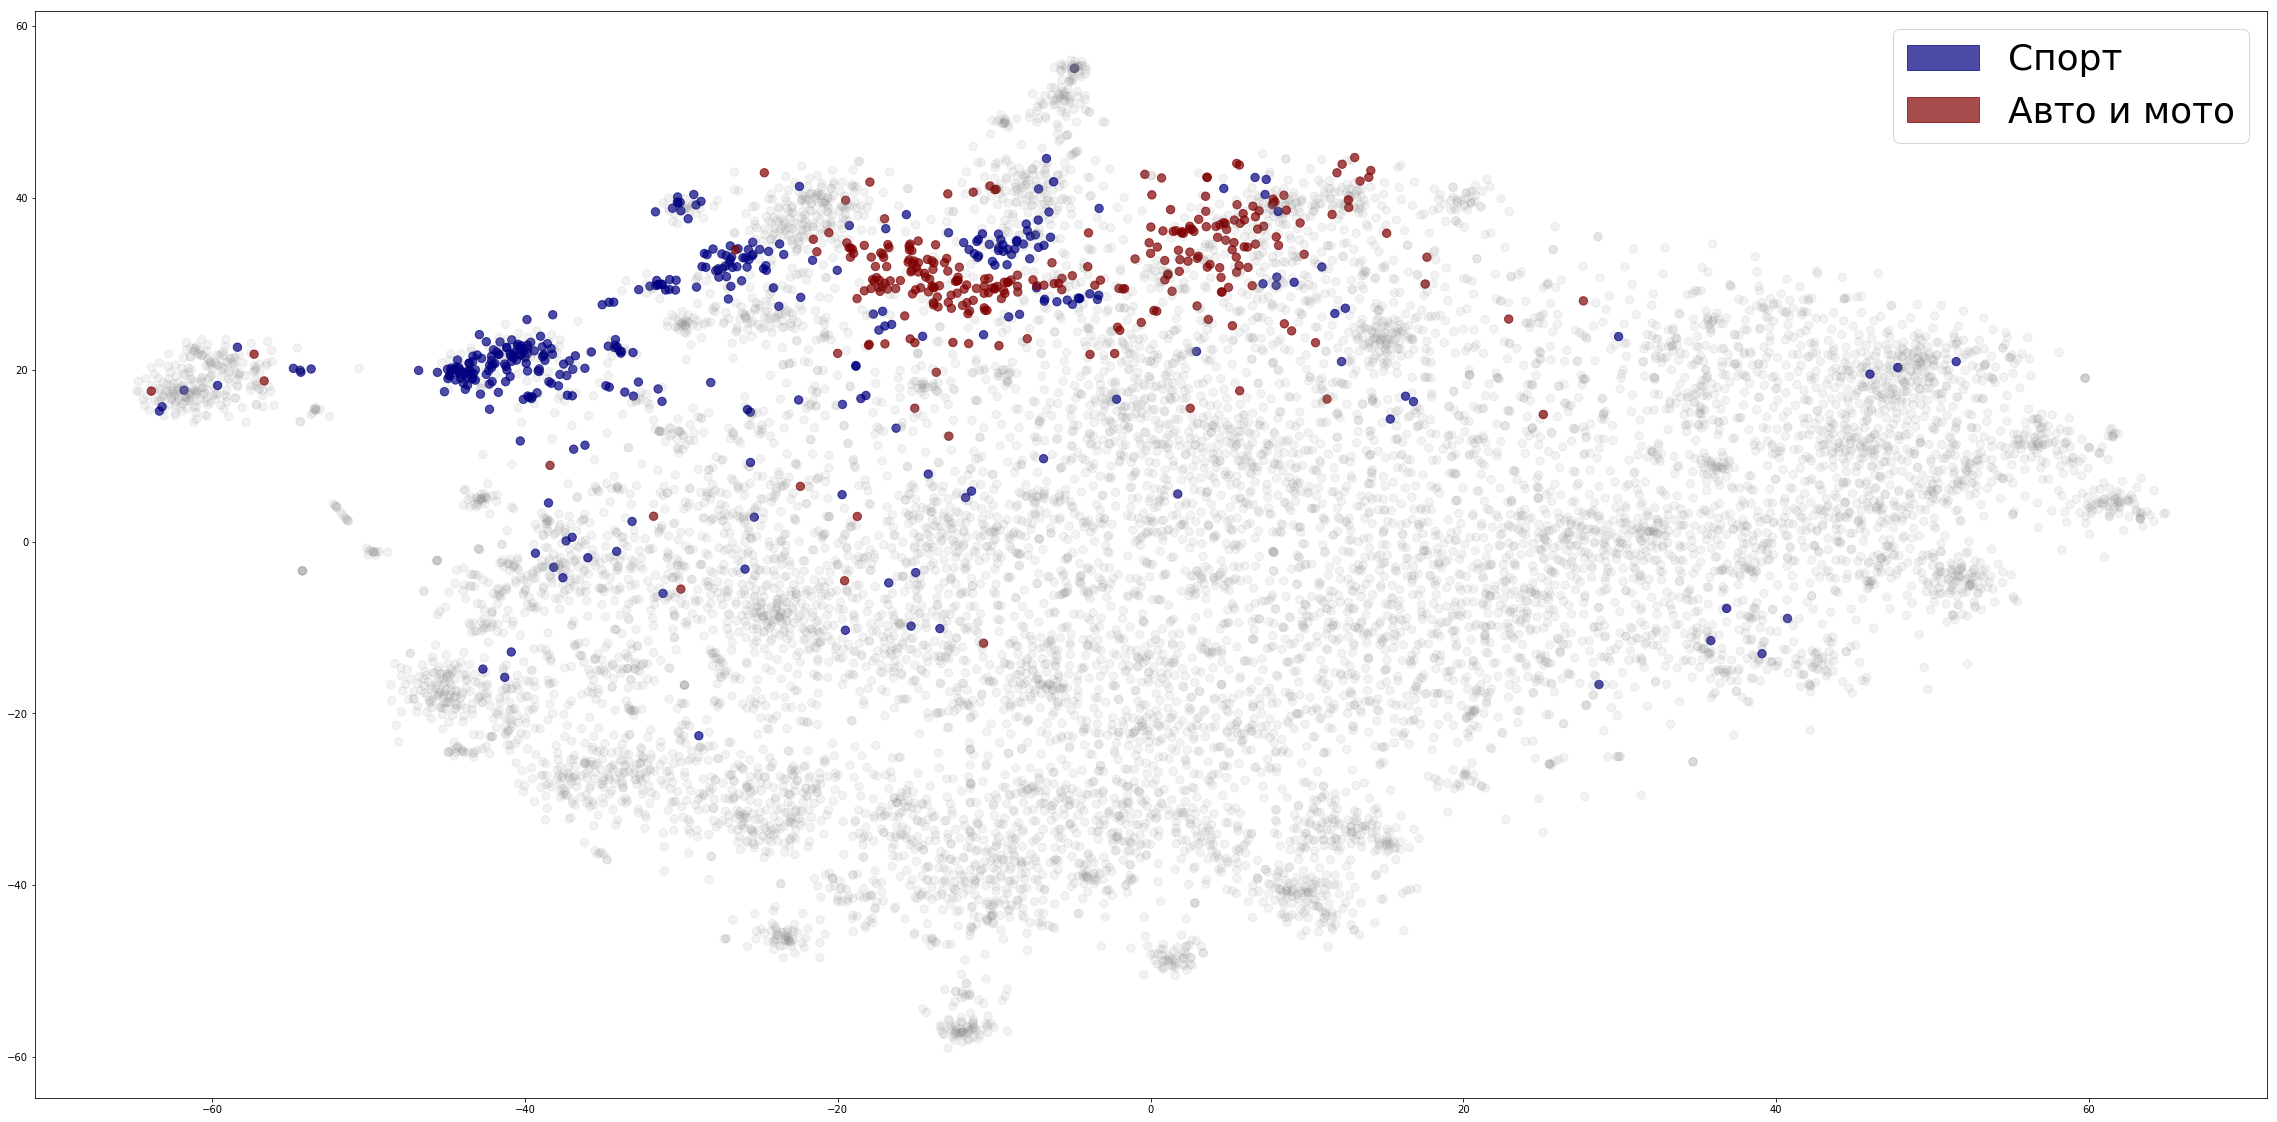
\includegraphics[width=1\textwidth]{index0}
\label{pic:categories}
\end{figure}

Полученное изображение наглядно показывает, что обученная модель действительно получает семантически похожие векторы. Так, сообщества с одинаковыми категориями находятся рядом друг с другом. Интересно, что различные сообщества, интересующие мужскую аудиторию социальной сети, находятся достаточно близко друг к другу. Кроме того, на рисунке можно заметить несколько небольших скоплений сообщества с категорией <<Спорт>>, относящиеся к разным видам спорта.  

Дополнительно был обучен алгоритм кластеризации k-means на результирующих многомерных векторах. Было проведено разбиение на 32 кластера, мною была проведена ручная разметка нескольких из них. (см. рис. \ref{pic:clusters})

\begin{figure}[h]
\caption{Визуализация векторного пространства}
\centering
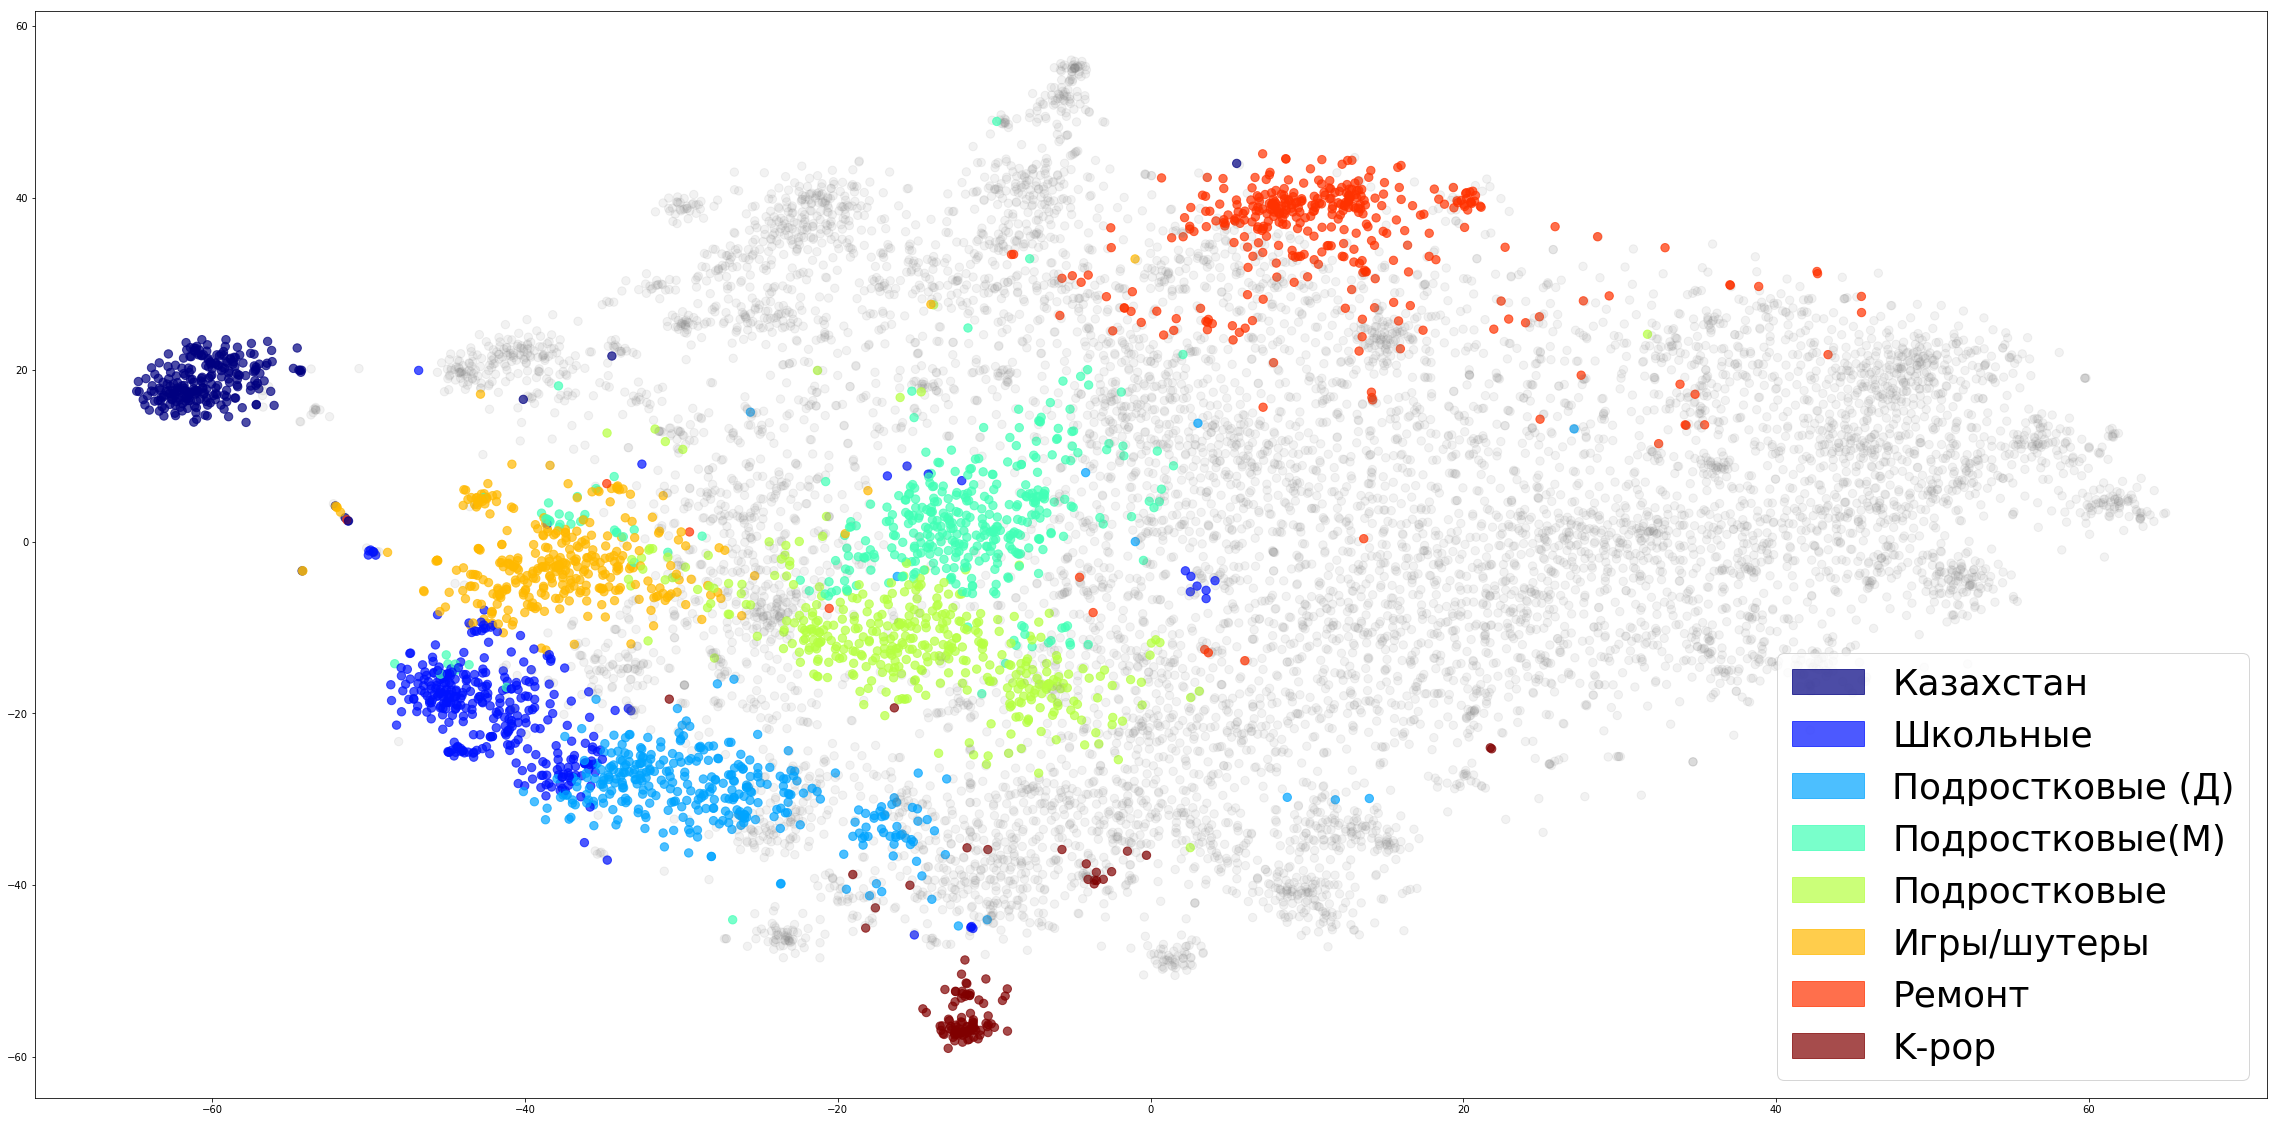
\includegraphics[width=1\textwidth]{clusters}
\label{pic:clusters}
\end{figure}

На рисунке видно, что алгоритм сохраняет важные свойства сообществ. К примеру, в социальной сети существует большое число пользователей из Казахстана, которые создают сообщества, записи в которых ведутся на казахском языке. Заметим, что кластер таких сообществ заметно удалён от общей картины. 

Возрастные категории пользователей сообществ также учитываются, сообщества тематик, интересующих пользователей школьного возраста расположены рядом с сообществами подростковых тематик, а так же рядом с кластером компьютерных игр. Интересно, что сообщества, которые интересуют юношей, находятся в некотором отдалении от сообществ, привлекающих аудиторию девушек. В то же время оба кластера находятся в близости к кластеру школьных тематик.

Отдельно стоит отметить кластер специфических, но популярных, интересов пользователей, которым является кластер с корейской поп-музыкой (K-pop). Кластер таких сообществ стоит в некотором отдалении от всех остальных, и достаточно близко к сообществам для молодых девушек. Интересно, что согласно интернет-опросам, основная демография слушателей корейской музыки --- молодые девушки.

Сообщества, относящиеся к ремонту, лежат на карте близко с сообществам спортивной и авто тематик (см. рис. \ref{pic:categories}), показывая популярность таких сообществ у мужской части пользователей социальной сети.    

\chapterconclusion

Эксперименты показали, что полученные вектора действительно отвечают главному требованию --- они сохраняют семантический смысл сущностей (сообщества социальной сети). Было показано, что предлогаемый алгоритм работает лучше, чем альтернативные варианты. Дополнительным приемуществом модели является меньшая требовательность к ресурсам оборудования, на котором она обучается. 

Использование полученных векторов в моделях машинного обучения для решения спектра различных задач показало, что полученные векторы могут быть применены на практике в других алгоритмах. Кроме того, гибкость алгоритма и возможность работать с различными типами данных позволяет использовать конкретную модель получения векторов, подстраиваясь под условия задачи. Эксперимент показал, что различные вариации модели позволяют лучше решать задачи, в зависимости от их контекста. 


%% Макрос для заключения. Совместим со старым стилевиком.
\startconclusionpage

В данной работе был предложен алгоритм выделения векторного представления сообществ на основе сессионных действий пользователя. Было предложено 3 вариации конечной модели, для работы с подписками и отписками пользователей (п. \ref{sec:algo-subs}), лайками пользователей (п. \ref{sec:algo-likes}) и комбинированный подход, учитывающий оба типа событий (п. \ref{sec:algo-combined})

Экспериментально было показано, что полученные алгоритмы могут быть применены для решения других задач, таких как классификация сообществ по признакам (категория или геолокация), предсказание следующего действия пользователя (может быть использовано в рекомендательных системах), кластеризация сообществ (может быть использовано для рекламы сообществ).

3 вариации алгоритма показывают гибкость модели, и, как показывают эксперименты, разные вариации алгоритма могут быть успешно использованы в различных задачах. 

Модель в дальнейшем может быть расширена на более широкий спектр действий пользователей (слабых событий, таких как клики пользователя на сообщества) 

%% TODO

\printmainbibliography

%% После этой команды chapter будет генерировать приложения, нумерованные русскими буквами.
%% \startappendices из старого стилевика будет делать то же самое
\appendix

\end{document}
